\subsection{Pre-Commit SA}

\sidebyside{0.5}{
  Simple Definitions

  \begin{itemize}

    \setlength\parskip{1em}

    \item Broadcast control: Advisory Bullseye Pictures only, no commit
      control, one airspace controller

    \item Tactical Control: Control is per Flight rather than broadcast and may
      contain both Bullseye and BRAA on the Agency frequency

    \item Close Control: Control is per flight, contains only BRAA and includes
      all instructions on the flight channel Pri/Forward (signified by AIC
      calling "MY SEPARATION" and released with "YOUR SEPARATION")

  \end{itemize}
}{%
  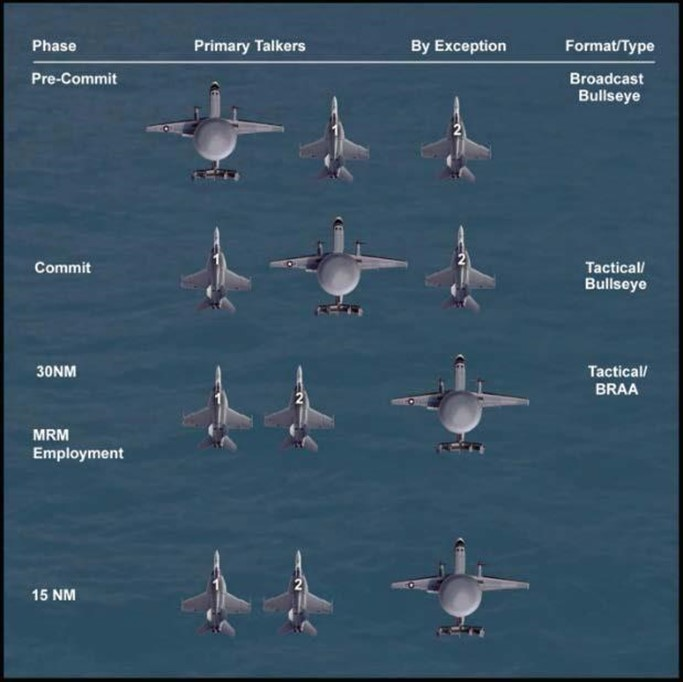
\includegraphics[width=\textwidth,align=t]
    {bvr/pre-commit-sa}%
}

\subsubsection*{General}

Once on station or enroute and fenced in but not committed, the flight requires
to perform these items.

\begin{itemize}

  \item Setup a scanning contract (see SOP)

  \item Mate radars

  \item Ensure the AIC is considering your TID's limited Bullseye capability
    (respectively the imprecision of NAV GRID's Voice Codes)"

\end{itemize}

\newpage

\subsubsection*{Process}

We recommend a default contract of FL takes High and WM takes Low fits for a
high low scan and any directions needing to be specifically mentioned.

Mate Radars at Flights altitude and cross over by 5 thousand feet.

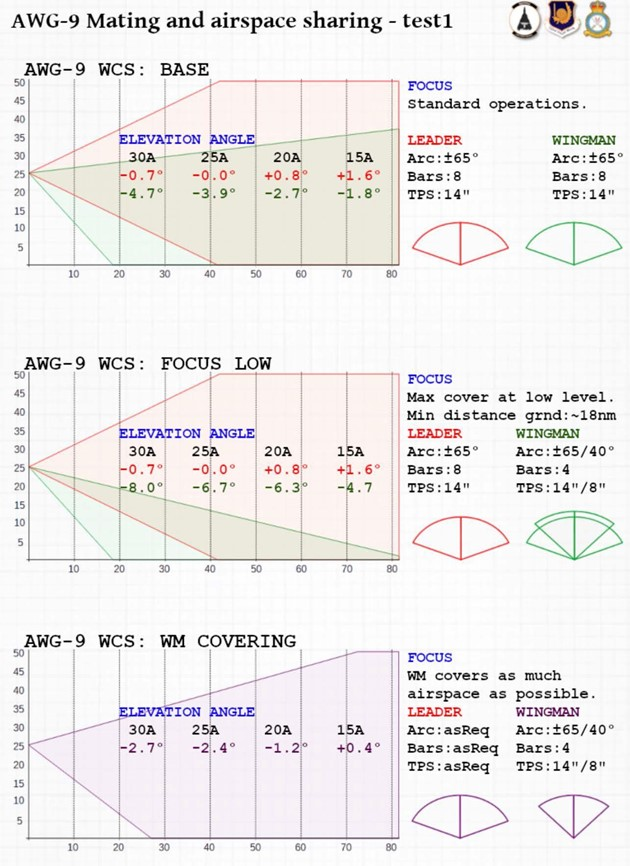
\includegraphics[width=\textwidth]{bvr/radar-mating}

A detailed Mating diagram with multiple options can be found in
\fullref{sec:radar-mating}

\subsubsection*{Examples}

\textbf{FL RIO (Pri)}: "Flight, Mate radars 50nm, 2 scan low from 15
thousand."

\textbf{FL RIO (Aux)}: "Magic, Spectre 1, request Tactical control via BRAA"
